% F5 DRAFT v0 (18 Oct 2026). All numbers in tables/figure are regenerated from raw logs by hesap_ham.py (no hand-typed results in tab_*.tex).
% Text numbers below were copied from sayilar.json; if you change an experiment, rerun hesap_ham.py and re-check the text.
% To submit to TMLR: replace the preamble by the official template (tmlr.sty) and keep the body.
\documentclass[11pt]{article}
\usepackage[utf8]{inputenc}
\usepackage[T1]{fontenc}
\usepackage{lmodern}
\usepackage[margin=1in]{geometry}
\usepackage{booktabs,graphicx,amsmath,amssymb,microtype,xcolor}
\usepackage[numbers,sort&compress]{natbib}
\usepackage[hidelinks]{hyperref}
\newcommand{\todo}[1]{{\color{red}[TODO: #1]}}
\title{How much compute do bundled training tricks save for small language models? A preregistered scale ladder on one laptop GPU (0.4M--85M parameters)}
\author{Mert Y\"unl\"u\\Independent researcher, Ankara, T\"urkiye\\\texttt{mert.yunlu08@gmail.com}}
\date{Draft v0, 18 October 2026}
\begin{document}
\maketitle

\begin{abstract}
Many training tricks are reported to save 1.4--2$\times$ compute, but such claims are often measured against untuned baselines and at a single scale.
On a single 8~GB laptop GPU we measure how much compute a bundle of known tricks (canon layers, Muon-type optimizers, QK-norm, hashed bigram embeddings, a warmup-stable-decay schedule, and depth growth) saves for GPT-style models from 0.4M to 85M non-embedding parameters.
Rules for passing and killing a variant were written before the runs, and the baseline's learning rate was tuned.
Our metric is the compute multiplier $m$: how many times more FLOPs the tuned baseline needs to reach the same validation loss.
The best recipe reaches the baseline's loss with $m\approx2.3$--$2.7$ at 25M--85M parameters under the baseline's local scaling slope ($m\approx1.8$--$2.0$ under the steeper slope of our small ladder), but the gain does not grow with scale: the relative loss reduction at equal tokens falls from about 10\% (1.3M) to 5\% (7.4M), 4.1\% (25M), 3.9\% (49M) and 3.1\% (85M); the two largest sizes are single runs.
Tuning the baseline's learning rate alone is worth $1.25$--$1.5\times$ compute at 25M--85M.
Of eight variants added to the base recipe, three were killed by preregistered rules, three gave no gain and two passed; twelve earlier variants are reported as well.
We also document pitfalls in our own pipeline (a checkpoint-resume bug, an invalid mixture-of-experts arm, inconsistent slope conventions across internal reports) and list what this study does not show.
\end{abstract}

\section{Introduction}
Training-efficiency papers regularly report that a new optimizer, architecture tweak or schedule matches a baseline with 1.4--2$\times$ less compute.
Two methodological problems make such numbers hard to trust: baselines whose hyperparameters were not tuned as carefully as the proposed method's, and measurements at one scale.
\citet{wen2025fantastic} showed on 0.1B--1.2B models that carefully tuned AdamW baselines shrink the speed-ups of ten optimizers, down to about 1.1$\times$ at 1.2B.
\citet{kaddour2023notrain} found that gains of several efficient-training algorithms vanish against a baseline with a fully decayed learning rate.

We ask a narrow question at a scale reachable on a consumer laptop: \emph{for a bundle of recent tricks, how much compute is saved against a tuned baseline, and does the saving change as the model grows from 0.4M to 85M parameters?}
We make four contributions.
(i) A protocol: a ladder of model sizes at a fixed 20 tokens per parameter, a tuned baseline, a compute-multiplier metric with an explicit slope sensitivity analysis, and kill rules written before the runs.
(ii) Measurements: the best recipe saves about 1.8--2.7$\times$ compute (depending on the scaling slope) against the tuned baseline at 25M--85M parameters, but the relative loss advantage at equal tokens shrinks with size.
(iii) Negative results: several variants did not help and are reported.
(iv) A candid list of pipeline errors and limitations.
Almost all code was written by AI coding agents under the author's direction (Section~\ref{sec:ai}); every number here is regenerated from raw run files by a script that does not reuse the pipeline's own reporting code.

\section{Related work}
\textbf{Optimizer comparisons.}
\citet{wen2025fantastic} and \citet{semenov2025benchmarking} benchmark optimizers under tuned baselines; the former finds matrix-based optimizers' speed-up falls with model size.
\citet{qiu2025transfer} argue that with proper hyperparameter transfer ($\mu$P-style learning-rate scaling, blocking or spectral normalisation, and scaled independent weight decay) the gains of matrix-preconditioned optimizers such as Muon, SOAP and Shampoo can be kept across scales.
\citet{wen2026hyperball} attribute the shrinking gain to constant decoupled weight decay and propose Hyperball (fixed Frobenius norms of weights and updates), reporting 20--30\% token-equivalent speed-ups on Qwen3-style models up to 1.2B.
\citet{everett2026memory} show that relative optimizer performance and optimal hyperparameters change with training horizon at 51M--253M parameters.
\textbf{Model growth.}
\citet{du2024stacking} study depth stacking for LLM pre-training, and \citet{bu2025depth} propose zero/one-layer progressive training, reporting roughly 5$\times$ acceleration on GPT-2 with a theory-motivated expansion schedule.
\textbf{Architecture components.}
Canon layers \citep{allenzhu2025canon}, large hashed input vocabularies \citep{huang2025overtok}, QK-normalization and the warmup-stable-decay schedule \citep{hagele2024scaling,hu2024minicpm} are among the components of our recipes; Muon \citep{jordan2024muon,liu2025muon} is the base of the optimizer variants.
\textbf{Methodology.}
\citet{gundlach2025origin} show that algorithmic-progress estimates depend strongly on scale and baseline, and \citet{wortsman2023small} motivate small-scale proxies for large-scale phenomena.
Compute-optimal sizing follows \citet{kaplan2020scaling,hoffmann2022chinchilla}.
We did not find a ladder of this kind, with an explicit tuned baseline and preregistered kill rules, for the combination of components studied here at $\le$100M parameters; our literature search was not exhaustive and we claim no priority.

\section{Setup}
\subsection{Models, data and training}
All models are pre-norm GPT-style transformers (RMSNorm, RoPE, GELU MLP with 4$\times$ expansion, head dimension 64, untied embeddings, vocabulary 8{,}192, context 512).
We call $N$ the number of non-embedding parameters.
\emph{Small ladder:} 2$\times$128, 3$\times$192, 4$\times$256 and 6$\times$320 (layers$\times$width) with $N$ = 0.39M, 1.33M, 3.15M and 7.4M (g1--g4); 32{,}768 tokens per step.
\emph{Main ladder:} 8$\times$512 (25.2M), 10$\times$640 (49.2M) and 12$\times$768 (85.0M); 131{,}072 tokens per step.
Every run sees $20N$ tokens (one pass, no repetition: 0.38B tokens cached for the small ladder, a 4B-token stream for the main ladder) of the ClimbMix web corpus \citep{diao2025climb}\footnote{ClimbMix (Nemotron-ClimbMix, 400B tokens) is introduced in the cited paper; we use the shuffled copy released on the Hugging Face Hub as \texttt{karpathy/climbmix-400b-shuffle}.}; all arms see the same token order.
The validation loss is measured at the end of training on a held-out shard (2M tokens for the small ladder, 1M for the main ladder), in nats per token.
Training uses bf16 autocast, gradient clipping at 1.0, AdamW $(0.9,0.95)$ with weight decay 0.1 for the baseline, 2\% warmup and cosine decay to 10\% of the peak.
The peak learning rate rule is $1.5\cdot10^{-3}\cdot256/d$ times a multiplier (``LR$\times$1'' is the default).
All runs use one RTX~4060 Laptop GPU (8~GB); the main ladder used \texttt{torch.compile}.

\subsection{Compute accounting and the multiplier \texorpdfstring{$m$}{m}}
Compute is $C=6\,(N_{\text{body}}+V d)\,D$ FLOPs, where $D$ is the number of training tokens, $V d$ is the output head, and growth runs are charged with their half-depth body for the first half of training.
Embedding lookups, hashed-table memory and optimizer-state arithmetic (e.g.\ Newton--Schulz iterations) are not counted (Section~\ref{sec:threats}).
For a run $r$ and a baseline $b$ at the same size, assuming the baseline's final loss follows a local power law $L\propto C^{-s}$ along the 20-tokens-per-parameter ladder,
\begin{equation}
m \;=\; \frac{C_b}{C_r}\Big(\frac{L_b}{L_r}\Big)^{1/s},
\end{equation}
i.e.\ the factor by which the baseline's compute would have to be multiplied to reach the loss of $r$.
The slope $s$ is the central modelling choice: only three baseline points exist per ladder, so no irreducible-loss term can be fitted and $s$ carries no confidence interval.
We therefore also report a slope-free quantity, the \emph{gap} $(L_b-L_r)/L_b$ at equal tokens, which ignores that growth recipes use fewer FLOPs ($c=C_b/C_r>1$).
Preregistered choices were: $s$ from the default-LR baseline points of the same ladder (0.0595 for the main ladder); in this paper we additionally report the tuned baseline's own local slope $s=0.0548$ and the small ladder's $s=0.0932$ (default baseline) as a sensitivity band, a post-hoc addition.

\subsection{Recipes and baselines}
\textbf{Baseline.} AdamW, cosine schedule. The \emph{default} baseline uses LR$\times$1; the \emph{tuned} baseline uses the best learning-rate multiplier we found: LR$\times$2.0 for the small ladder (grid LR$\in\{0.7,1,1.4,2\}$, weight decay $\in\{0.05,0.1,0.2\}$, partially crossed, tuned at g3/g4), and LR$\times$2.8 for the main ladder (25M: $\{1,2,2.8\}$; 49M and 85M: $\{1,2.8\}$).
\textbf{Recipe A} (``paket'' in our logs): depthwise causal convolutions of width 4 at the attention and MLP inputs (canon layers), Muon for hidden weight matrices with decoupled weight decay 0.1 and update RMS matched to AdamW (``MuonW''), QK-norm, a zero-initialised hashed bigram embedding (131{,}071 rows), and a warmup-stable-decay schedule (constant, then linear decay to 10\% over the last 45\% of steps); LR$\times$1.
\textbf{Recipe B} (``paket2''): Recipe A with MuonW replaced by Hyperball ($\eta=0.008$, our implementation from the description in \citet{wen2026hyperball}) and depth growth (start at half depth; at 50\% of the steps each block is duplicated in place and optimizer state is copied); LR$\times$2.8 (chosen at g3 from $\{1.4,2,2.8\}$).
Further details are in Appendix~\ref{app:recipe}.

\subsection{Preregistration}
Before the runs we wrote, in dated files with SHA-256 hashes, the metric, the sizes, the variants, pass rules ($a_4=m(\text{variant})/m(\text{Recipe A})\ge1.05$ at the largest small size), kill rules ($a_4<1$), seed requirements, and the transfer rule for the final 85M run: $m\ge2$ ``preserved'', $1.1\le m<2$ ``shrinking'', $m<1.1$ ``vanished'' (Appendix~\ref{app:prereg}).
Deviations are listed in Appendix~\ref{app:dev}.

\section{Results}
\subsection{Tuning the baseline matters}
Against the default baseline, tuning only the learning rate lowers the final loss by 2.4\% at 25M (3.2538$\to$3.1759), 1.4\% at 49M and 1.3\% at 85M, which corresponds to $m=1.50$, $1.27$ and $1.25$ (slope 0.0595).
In the small ladder the Recipe A multiplier at g4 falls from 2.21 to 1.79 when the tuned baseline is used.
The optimum LR$\times$2.8 lies at the edge of the grid at 25M, so the tuned baseline is itself probably under-tuned.

\subsection{Main ladder}
Table~\ref{tab:main} and Figure~\ref{fig:m} summarise the 25M--85M runs.
Against the tuned baseline, Recipe B reaches $m=2.73$ and $2.68$ (two seeds) at 25M, $2.69$ at 49M and $2.32$ at 85M under the baseline's local slope.
Recipe A is flat across 25M and 49M ($2.08/2.10$ and $2.07$).
The slope-free gap tells the same story: Recipe B 4.1\% / 3.9\% / 3.1\% and Recipe A 3.9\% / 3.9\% at 25M / 49M / 85M.
The 85M drop (0.8--0.9 percentage points, 0.030 nat relative to 49M) is large compared with the seed spread we measured at 25M (0.003 nat, i.e.\ 0.1 points), but 49M and 85M are single runs and the baseline learning rate was not re-tuned at these sizes.
Over the whole range from 1.3M to 85M the gap falls roughly monotonically (Figure~\ref{fig:m}b), although the small and main ladders differ in batch size, validation set and tuned-LR multiplier.
\begin{figure}[t]\centering
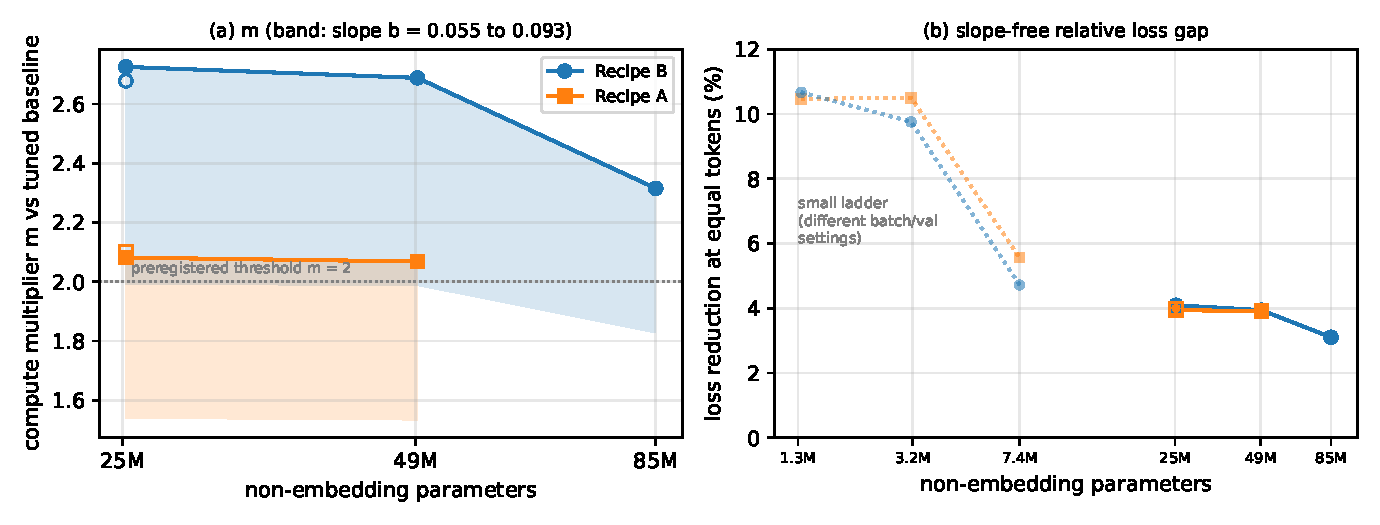
\includegraphics[width=\linewidth]{fig_m_size.pdf}
\caption{(a) Compute multiplier $m$ against the tuned baseline for the main ladder; line: baseline-local slope ($s=0.0548$); band: slopes up to 0.0932; open markers: second seeds at 25M. (b) Relative loss reduction at equal tokens (slope-free); dotted: small ladder, tuned baseline LR$\times$2.0.}\label{fig:m}
\end{figure}
%% generated by hesap_ham.py (do not edit by hand)
\begin{table}[t]\centering\small
\caption{Main ladder (25M--85M non-embedding parameters, 20 tokens/parameter, one run per cell unless noted). Loss is the final validation loss (nats/token, 1M held-out tokens); $m$ is the compute multiplier against the \emph{tuned} baseline (AdamW, LR$\times$2.8). $m$ uses the baseline's own local slope $b=0.0548$; the bracket is the range for $b\in[0.0548,0.0932]$. ``gap'' is the relative loss reduction at equal tokens (slope-free).}\label{tab:main}
\begin{tabular}{llrrrr}\toprule
Size & Run & Loss & $m$ [range] & FLOP ratio $c$ & gap (\%) \\ \midrule
25M & baseline, default LR & 3.2538 & -- & -- & -- \\
 & baseline, tuned LR & 3.1759 & 1 & 1 & 0 \\
 & Recipe A & 3.0507 & 2.08 [1.54--2.08] & 0.999 & 3.9 \\
 & Recipe A (seed 2) & 3.0492 & 2.10 [1.55--2.10] & 0.999 & 4.0 \\
 & Recipe B & 3.0460 & 2.73 [1.99--2.73] & 1.271 & 4.1 \\
 & Recipe B (seed 2) & 3.0489 & 2.68 [1.97--2.68] & 1.271 & 4.0 \\
\midrule
49M & baseline, default LR & 3.0085 & -- & -- & -- \\
 & baseline, tuned LR & 2.9660 & 1 & 1 & 0 \\
 & Recipe A & 2.8500 & 2.07 [1.53--2.07] & 0.999 & 3.9 \\
 & Recipe B & 2.8491 & 2.69 [1.99--2.69] & 1.291 & 3.9 \\
\midrule
85M & baseline, default LR & 2.8292 & -- & -- & -- \\
 & baseline, tuned LR & 2.7919 & 1 & 1 & 0 \\
 & Recipe B & 2.7052 & 2.32 [1.83--2.32] & 1.302 & 3.1 \\
\bottomrule\end{tabular}\end{table}


\subsection{Slope sensitivity and the preregistered transfer rule}
The preregistered 85M rule (using the default baseline's S1--S3 slope, 0.0595) gave $m=2.77$ against the default and $2.21$ against the tuned baseline, both ``preserved''.
Because $m$ depends on $s$, Table~\ref{tab:sens} shows how it changes: the threshold $m\ge2$ is met at 85M only if $s\le0.0735$; with the small-ladder slope (0.0932) the multiplier is 1.83 (``shrinking'').
We have no way to decide between slopes with three baseline points per ladder; the slope-free gap, which does not depend on it, decreased.
%% generated by hesap_ham.py (do not edit by hand)
\begin{table}[t]\centering\small
\caption{Sensitivity of $m$ (tuned baseline) to the slope $b$ used in $m=c\,(L_{\rm base}/L)^{1/b}$. The threshold $m\ge2$ of the preregistered transfer rule is met at 85M only for $b\le0.0735$.}\label{tab:sens}
\begin{tabular}{lrrrrrrrr}\toprule $b$ & 0.0450 & 0.0500 & 0.0548 & 0.0595 & 0.0700 & 0.0800 & 0.0932 & 0.1000 \\ \midrule
25M Recipe B & 3.22 & 2.93 & 2.73 & 2.57 & 2.31 & 2.14 & 1.99 & 1.93 \\
49M Recipe B & 3.15 & 2.88 & 2.69 & 2.54 & 2.29 & 2.13 & 1.99 & 1.93 \\
85M Recipe B & 2.62 & 2.45 & 2.32 & 2.21 & 2.04 & 1.93 & 1.83 & 1.79 \\
\bottomrule\end{tabular}\end{table}


\subsection{Small ladder}
Table~\ref{tab:small} gives the 1.3M--7.4M results.
Both recipes give $m\approx3.1$--3.4 against the tuned baseline at g2 and g3 but only $1.8$--$2.0$ at g4, and the equal-token gap falls from about 10\% to 5\%.
The g2--g4 slope of the tuned small-ladder baseline is 0.097.
Seeds 1 and 2 agree to within 0.03 in $m$.
%% generated by hesap_ham.py (do not edit by hand)
\begin{table}[t]\centering\small
\caption{Small ladder (non-embedding parameters: g2 1.3M, g3 3.2M, g4 7.4M). $m$ against the default-LR baseline (slope $b=0.0932$) and against the tuned baseline (LR$\times$2.0, slope $b=0.0973$). Seeds 1 and 2 where run.}\label{tab:small}
\begin{tabular}{llcrrr}\toprule
Recipe & Size & Seed & $m$ (default baseline) & $m$ (tuned baseline) & gap vs tuned (\%) \\ \midrule
Recipe A & g2 & 1 & 3.41 & 3.10 & 10.5 \\
Recipe A & g3 & 1 & 4.90 & 3.11 & 10.5 \\
Recipe A & g3 & 2 & 4.88 & 3.10 & 10.5 \\
Recipe A & g4 & 1 & 2.21 & 1.79 & 5.6 \\
Recipe A & g4 & 2 & 2.19 & 1.78 & 5.5 \\
\midrule
Recipe B & g2 & 1 & 3.78 & 3.43 & 10.7 \\
Recipe B & g3 & 1 & 5.27 & 3.36 & 9.8 \\
Recipe B & g3 & 2 & 5.23 & 3.34 & 9.7 \\
Recipe B & g4 & 1 & 2.46 & 2.01 & 4.7 \\
Recipe B & g4 & 2 & 2.45 & 2.00 & 4.7 \\
\bottomrule\end{tabular}\end{table}


\subsection{Variants that did not make the recipe}
Table~\ref{tab:cand} lists the variants added to Recipe A.
Hyperball alone was killed ($a_4=0.917$), but combined with growth it passed in two seeds and became Recipe B; growth alone also passed.
Hashed 2/3-gram inputs, learned prefix tokens and a deeper-thinner shape gave no gain; a masked hybrid objective and learnability-based example selection were killed.
A mixture-of-experts arm is not reported because of an implementation error (Appendix~\ref{app:dev}).
Plain (non-decayed) Muon collapsed at g4 ($m=0.52$) and was replaced post hoc by MuonW.
A first generation of twelve variants (curricula, multi-token prediction, a flat low-learning-rate schedule, data pruning, loss weighting, looped depth and others) was run on the small ladder before the recipes were assembled; the outcomes, including the many kills, are in Appendix Table~\ref{tab:first}.
%% generated by hesap_ham.py (do not edit by hand)
\begin{table}[t]\centering\small
\caption{Ablations added to Recipe A (seed 1; $a_k=m(\text{variant})/m(\text{Recipe A})$ at size $g_k$, default-LR baseline). Preregistered rules: pass if $a_4\ge1.05$; kill if $a_4<1.0$.}\label{tab:cand}
\begin{tabular}{lrrrl}\toprule Variant & $a_2$ & $a_3$ & $a_4$ & Verdict \\ \midrule
Hyperball instead of MuonW & 0.877 & 0.898 & 0.917 & killed \\
growth (half depth $\to$ full at 50\%) & 1.288 & 1.155 & 1.153 & passed \\
Hyperball + growth (= Recipe B) & 1.061 & 1.054 & 1.101 & passed (a$_4\ge$a$_3$ in 2 seeds) \\
hashed 2/3-gram input embeddings & 1.019 & 1.026 & 1.032 & no gain \\
4 learned prefix tokens & 1.250 & 1.009 & 1.023 & no gain \\
deeper-thinner (1.5$\times$ layers) & 1.490 & 1.041 & 1.033 & no gain \\
masked+causal hybrid objective & 0.652 & 0.616 & 0.600 & killed \\
learnability-based example selection & 0.530 & 0.506 & 0.540 & killed \\
\bottomrule\end{tabular}\end{table}

A repetition control (a quarter of the unique data repeated four times) cut Recipe A's advantage over the baseline in the same repeated-data setting from $4.9\times$ to $2.5\times$ at g3 and from $2.2\times$ to $1.4\times$ at g4.

\subsection{Synthetic reasoning and knowledge capacity (single seed)}
On synthetic tasks with exactly computable answers and longer chains at test time, Recipe A beats the baseline in out-of-distribution accuracy by 2.2, 6.9 and 7.5 points at three small sizes (Table~\ref{tab:reason}); a weight-tied looped variant gains most from extra passes at test time (pass 1$\to$4: +11.9, +22.6, +15.1 points) but does not consistently beat Recipe A at equal training compute.
On synthetic biographies Recipe A stores about 1.8--1.9$\times$ more bits per non-embedding parameter than the baseline (1.41 vs 0.74 single template; 1.49 vs 0.85 with five paraphrases), and paraphrases raise held-out QA accuracy (Table~\ref{tab:know}); in this tiny model the hashed bigram table enlarges the recipe's total parameter count about elevenfold, so the comparison is per non-embedding parameter only.
These are one-seed, tiny-model, synthetic experiments and do not support claims about general reasoning.
%% generated by hesap_ham.py (do not edit by hand)
\begin{table}[t]\centering\small\setlength{\tabcolsep}{3pt}
\caption{Synthetic reasoning tasks (exact-match accuracy, mean of 4 tasks, out-of-distribution = longer chains than seen in training). Equal training FLOPs; one seed.}\label{tab:reason}
\begin{tabular}{lrrrrrr}\toprule Size & Baseline OOD & Recipe A OOD & Loop OOD (2 passes) & Loop pass 1 & Loop pass 4 & A$-$base (pts) \\ \midrule
2$\times$128 & 0.407 & 0.428 & 0.417 & 0.188 & 0.307 & +2.2 \\
3$\times$192 & 0.403 & 0.471 & 0.486 & 0.204 & 0.430 & +6.9 \\
4$\times$256 & 0.407 & 0.482 & 0.456 & 0.259 & 0.410 & +7.5 \\
\bottomrule\end{tabular}\end{table}

%% generated by hesap_ham.py (do not edit by hand)
\begin{table}[t]\centering\small
\caption{Knowledge capacity on synthetic biographies (50k people, 53.2 bits each, 100 exposures, single run). Bits per non-embedding parameter and exact-match QA accuracy on held-out question halves.}\label{tab:know}
\begin{tabular}{llrrr}\toprule Phrasing & Model & Bits learned (M) & bits/param & QA acc. \\ \midrule
single template & baseline & 1.31 & 0.74 & 0.225 \\
single template & Recipe A & 2.50 & 1.41 & 0.857 \\
5 paraphrases & baseline & 1.51 & 0.85 & 0.331 \\
5 paraphrases & Recipe A & 2.65 & 1.49 & 0.999 \\
\bottomrule\end{tabular}\end{table}


\subsection{Downstream benchmarks}
At 85M, both Recipe B and the default baseline (the tuned baseline was not evaluated) are close to chance on MMLU, ARC-Challenge and TurkishMMLU and above chance on HellaSwag (about 0.35 against a chance level of 0.25) and ARC-Easy (0.48--0.51 against 0.25); the differences between the two arms are at most 3.6 points (ARC-Easy accuracy 0.512 vs 0.476; $n=1000$, standard error $\approx$1.6 points) and at most 1.2 points elsewhere, so we draw no conclusion from them.
The final validation bits-per-byte of Recipe B was 0.971, inside the band 0.915$\pm$0.175 that we had preregistered by extrapolating the small ladder 129$\times$ in compute, but on the pessimistic side of the point prediction.

\section{Threats to validity and limitations}\label{sec:threats}
\begin{enumerate}
\item \textbf{Baseline tuning is partial.} Only the learning rate (and weight decay on the small ladder) was tuned; $\beta_2$, warmup and batch size were not. At 25M the best learning-rate multiplier is at the grid edge; at 49M and 85M the multiplier was reused rather than re-tuned. Recipe A's learning rate was never tuned and Recipe B's was tuned at 3.2M only, so comparisons between recipes are confounded by tuning effort. Our $m$ values are therefore more likely over- than under-estimates \emph{for the recipe}, and the shrinking gap could partly reflect untuned learning rates at 85M.
\item \textbf{Seeds.} 49M and 85M are single runs; two seeds exist only at 25M (spread 0.0015--0.0029 nat, which corresponds to roughly $\pm5\%$ in $m$) and on the small ladder. No baseline was replicated.
\item \textbf{Scale and data.} Models are at most 85M parameters, trained on one English web corpus with one tokenizer; extrapolation beyond this range is not supported by our data.
\item \textbf{Slope choice} (Section~4.3): at 85M $m$ ranges from 1.83 to 2.32 over the plausible slopes (a 25\% spread), so $m$ is not well identified by our data; we therefore emphasise the slope-free gap.
\item \textbf{Compute accounting.} FLOPs follow $6ND$; they exclude embedding/hash-table memory (the bigram table adds $131{,}071\times d$ parameters: 67M at width 512, 100M at width 768) and Muon/Hyperball matrix iterations, which favours the recipes. Wall-clock hours (Appendix Table~\ref{tab:wall}) are indicative only (shared laptop, paused runs): they favour Recipe B by about 10\% at 49M and 85M and not at 25M.
\item \textbf{Numerical changes during the study.} The fast canon implementation (+10.4\% throughput, loss difference $\le0.0023$ nat in a 40-step check) was enabled from the 49M runs on; the small ladder compares eager-mode recipes with a compiled baseline (a 0.006 nat eager--compiled difference was measured once), which slightly under-states $m$ there.
\item \textbf{Post-hoc elements and multiple comparisons.} About two dozen variants were evaluated without multiplicity correction; MuonW and the choice of the middle slope values were added post hoc; the sensitivity band in this paper is post hoc. ``Passed'' means a sign, not a confirmed effect.
\item \textbf{Metric.} Validation loss only, final checkpoint; the only downstream evaluation is five multiple-choice benchmarks at 85M, with no conclusive difference between the arms.
\item \textbf{Implementation risk.} Most code was written by AI agents. We used bit-for-bit CPU comparisons of default code paths, positive controls and smoke tests, but no independent audit. Our Hyperball implementation follows the abstract of \citet{wen2026hyperball} and may differ from the authors' code.
\item \textbf{What this study does not show.} It does not show that the gains persist, grow or vanish beyond 85M; that any component is individually necessary; or that the recipe helps downstream capability.
\end{enumerate}

\section{Discussion}
Within 25M--85M our bundle saves roughly 2--2.7$\times$ compute against a learning-rate-tuned AdamW baseline, but the advantage in final loss is not growing with scale; it is flat from 25M to 49M and smaller at 85M, and it was much larger at 1--3M.
This is the same direction as \citet{wen2025fantastic} found for optimizers at larger scale, and is consistent with the hypothesis of \citet{wen2026hyperball} that fixed weight decay is one reason, which we did not test directly (Recipe B still wins at 85M; its Hyperball component alone lost at small sizes).
The most useful follow-ups are cheap relative to this study: second seeds at 49M and 85M, retuning of both arms' learning rates at 85M, and a $\mu$P-style transfer check.

\section{Statement on AI assistance and reproducibility}\label{sec:ai}
Most of the code and the experiment infrastructure were written and executed by AI coding agents (Claude, Anthropic) under the author's instructions.
The author set the goal and constraints (no pretrained weights, no distillation, one laptop), decided which experiments to run or stop, and reviewed the results; the first draft of this paper was also written with AI assistance.
All numbers in the tables and figure are regenerated from raw run files by \texttt{scripts/make\_report.py} in the repository, which re-implements the formulas independently and compared 137 values from the pipeline's own reports with 0 mismatches.
\textbf{Code, preregistration files and raw logs:} \url{https://github.com/latentcore/devrim-scale-ladder} (Apache-2.0).

\bibliographystyle{plainnat}
\bibliography{refs}

\appendix
\section{Recipe details}\label{app:recipe}
Muon: Nesterov momentum 0.95, five Newton--Schulz steps; MuonW: weight decay 0.1 and update scale $0.2\sqrt{\max(\text{rows},\text{cols})}$ so that AdamW's schedule and learning rate are reused; embeddings, output head, norms and the bigram table use AdamW at the baseline learning rate.
Hyperball: $R$ is the Frobenius norm of each 2-D block weight at its first step; each update is $W\leftarrow W-\eta R\,u/\|u\|_F$ followed by renormalisation to $R$, with no weight decay; $\eta$ scales with the learning-rate schedule.
Growth: the model starts with $\lceil L/2\rceil$ blocks and at step $\lfloor T/2\rfloor$ each block is copied in place ($1,1,2,2,\dots$); AdamW moments and Muon buffers are copied to the duplicates.
Canon: depthwise causal convolution, window 4, residual, applied before attention and before the MLP.
Peak learning rates before multipliers: $1.5\cdot10^{-3}\cdot256/d$ (e.g.\ $7.5\cdot10^{-4}$ at width 512).

\section{Preregistration documents}\label{app:prereg}
\begin{center}\small
\begin{tabular}{lll}\toprule
Document & Written & SHA-256 (prefix) \\ \midrule
Ladder, metric, small-ladder variants (Ek~1--6)$^\ast$ & 8 Oct 2026 & -- \\
Queue plan, kill rules, aggregation rules (Ek~7) & 12 Oct 12:56 & ed3cd1b6 \\
Reasoning exam sets and budget (Ek~7a) & 12 Oct 13:47 & 57107e5e \\
Knowledge-capacity settings (Ek~7b) & 12 Oct 13:51 & 129a6462 \\
Tuned baseline at 25M--85M (Ek~7c) & 12 Oct 15:53 & 89cd537a \\
85M run: predictions and decision rule & 16 Oct 17:11 & bc5d969a \\ \bottomrule
\end{tabular}\end{center}
$^\ast$Ek~3a, 5 and 6 were written after some small-ladder results were seen and are labelled post hoc in the files; Ek~1--4 preceded the runs they govern.
Ek~7c was written before any 25M run; its first hash (9a2c3a9f) belongs to the same text with the header time written as 16:40 and was superseded when the header was corrected to 15:50, before any related run (logged). The prefixes are SHA-256 values recorded in the timestamped queue log when each addition was written: for Ek~7--7c the text of the addition (from its heading to the end of its text, without trailing blank lines, separators or machine-generated markers), for the last row the whole file \texttt{KANIT\_ON\_KAYIT.md}. They can be re-checked with \texttt{prereg/verify\_hashes.py} in the repository.

\section{Deviations from the preregistered plan}\label{app:dev}
\begin{itemize}\itemsep0pt
\item \textbf{Mixture-of-experts arm invalid.} The 8-expert arm used about three times the intended token budget and exhausted the data at g4; it was stopped and is not reported.
\item \textbf{Lost grid point.} The Hyperball run with $\eta=0.004$ at 25M crashed after a pause because a restored RNG state was on the wrong device; the bug was fixed, but the $\eta$ grid at 25M lacks its lower edge ($\eta=0.008$ was selected among 0.008 and 0.016).
\item \textbf{Post-hoc MuonW.} Plain Muon collapsed at g4 and a weight-decayed variant was added after seeing this.
\item \textbf{Recipe B built by rule from passing arms.} Hyperball alone was killed, but the combination with growth passed in two seeds.
\item \textbf{Slope calibration instrument failed.} Two attempts to calibrate a scaling-exponent test (Transformer vs.\ LSTM) did not pass, so no exponent claims are made.
\item \textbf{Inconsistent slope conventions} in internal reports (0.0932, 0.0609, 0.0595); unified here.
\item \textbf{Time bookkeeping.} The run timer restarts after a pause, so recorded run times of paused runs are too short; wall-clock hours in Table~\ref{tab:wall} come from log timestamps. A helper figure in the 85M preregistration file (``0.8~h'', derived from such a timer) is wrong; the preregistered loss predictions are unaffected.
\end{itemize}

\section{First-generation variants}
%% generated by hesap_ham.py (do not edit by hand)
\begin{table}[t]\centering\small
\caption{First-generation variants on the small ladder (seed 1, $m$ against the default-LR baseline, slope $b=0.0932$; ``--'' = not run because an earlier gate failed). The recipes' components canon, MuonW (post hoc), QK-norm, bigram and WSD come from this stage.}\label{tab:first}
\begin{tabular}{lrrrl}\toprule Variant & g2 & g3 & g4 & Outcome \\ \midrule
flat low-LR schedule (LR$\times$0.1, init$\times$0.3) & 0.24 & 0.24 & 0.12 & killed \\
sequence-length curriculum & 1.03 & 1.01 & 0.86 & killed \\
multi-token prediction ($t{+}2$ head) & 0.58 & 0.70 & 0.78 & killed \\
data curriculum (easy to hard) & 0.99 & 0.95 & 0.87 & killed \\
probability-weighted loss (ZPD) & 0.31 & 0.27 & 0.22 & killed \\
data pruning (middle 50\%) & 1.00 & 1.07 & 1.00 & no gain \\
plain Muon (no weight decay) & 2.55 & 2.67 & 0.52 & collapsed at g4 \\
MuonW (added post hoc) & 1.22 & 2.05 & 1.40 & kept \\
canon layers alone & -- & 1.86 & 1.18 & kept \\
bigram soft targets & -- & 0.99 & -- & stopped at g3 gate \\
early growth (default LR) & -- & 1.07 & -- & stopped at g3 gate \\
looped depth (2 passes) & -- & 0.60 & -- & stopped at g3 gate \\
\bottomrule\end{tabular}\end{table}

\section{Wall-clock}
%% generated by hesap_ham.py (do not edit by hand)
\begin{table}[t]\centering\small
\caption{Wall-clock hours per run (from timestamps of the run log; the laptop was shared with other use and runs were paused/resumed, so these are indicative only).}\label{tab:wall}
\begin{tabular}{lrr}\toprule Size & tuned baseline & Recipe B \\ \midrule
25M & 1.9 & 2.0 \\
49M & 6.3 & 5.7 \\
85M & 15.9 & 14.2 \\
\bottomrule\end{tabular}\end{table}

\end{document}
